\hthree{Allgemein}

Für das Projektmanagement wird Github verwendet. Github bietet die Möglichkeit, einzelne Arbeitspakete zu erstellen und diese Meilensteinen und Unterprojekten Zuzuordnen. Dabei ist es möglich, dass der Status eines einzelnen Arbeitspaketes automatisch in die Spalten "To Do", "In Progress", "Review in progress", "Review approved" und "Done" verschoben wird.

\hthree{Erstellen eines Projektes}

Um ein Projekt zu erstellen, muss man zunächst ein Projekt im "Projects"-Tab (Abbildung \ref{fig:newProject}) erstellt werden.

\begin{figure}[H]
    \centering
    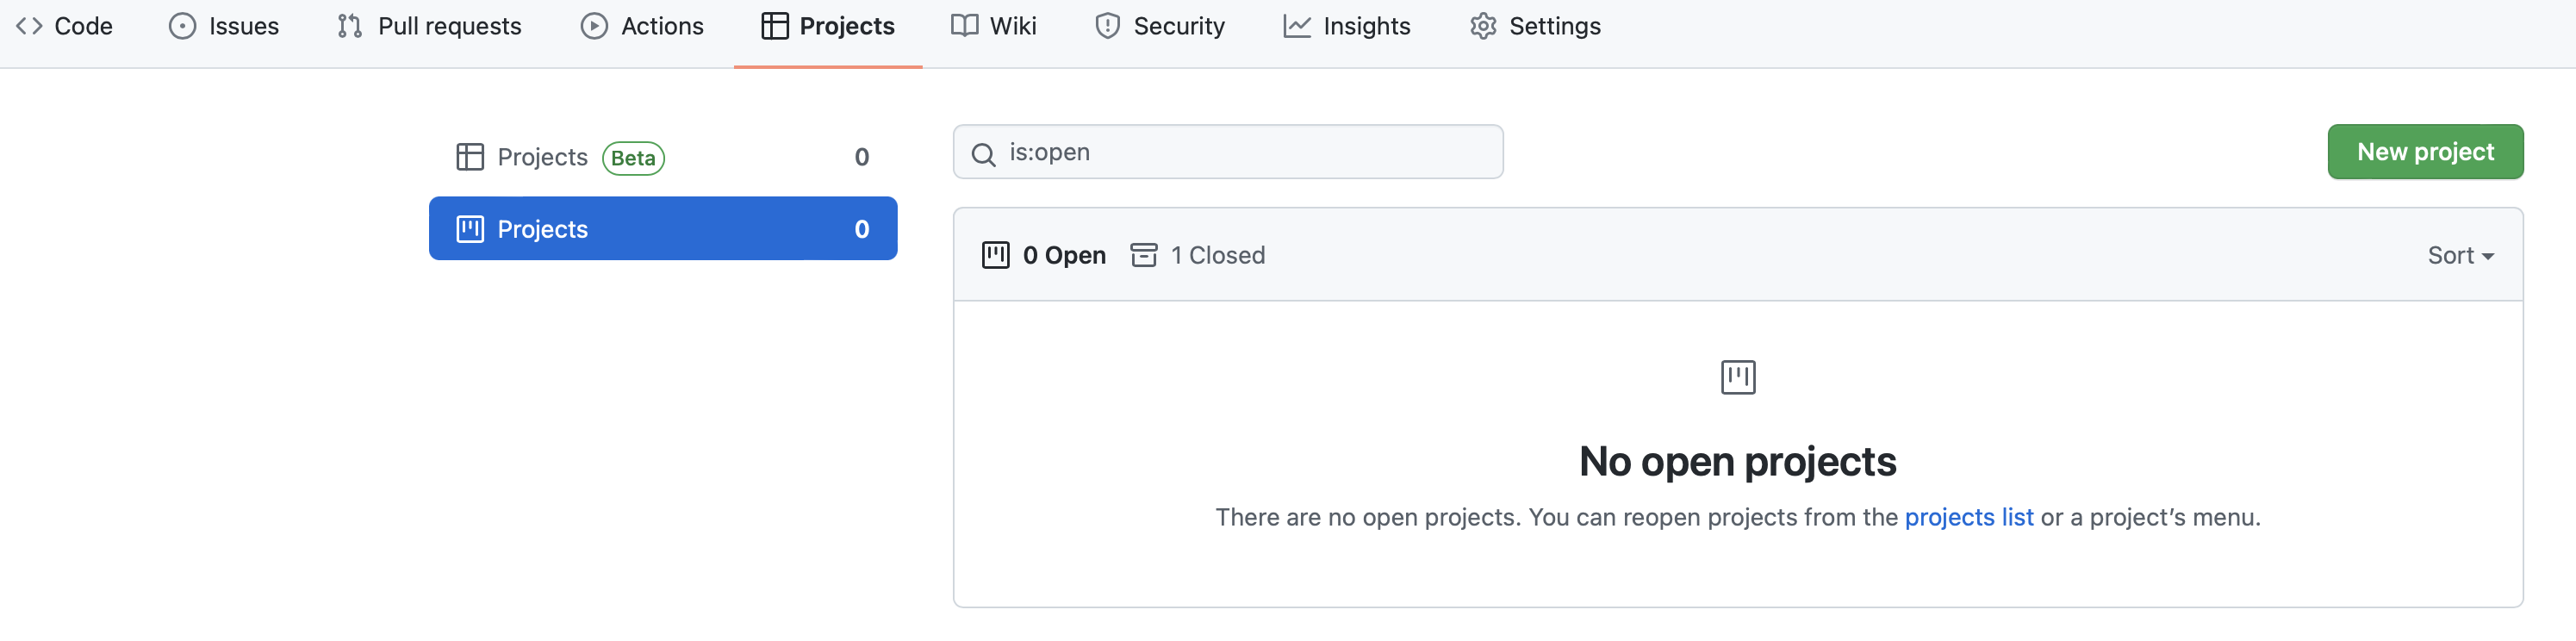
\includegraphics[width=\textwidth]{media/ProjectManagement/CreateProject.png}
    \caption{Github Projektübersicht mit "New Project" Button}
    \label{fig:newProject}
\end{figure}

Einem Projekt wird ein Name und eine Beschreibung zugewiesen. Außerdem muss das Projekt-"template" auf "Automated kanban with reviews" gesetzt werden, damit die Spalten "To Do", "In Progress", "Review in progress", "Review approved" und "Done" erstellt und die Verschiebung der Karten automatisiert wird. (Siehe Abbildung \ref{fig:enterProjectInfo})

\begin{figure}[H]
    \centering
    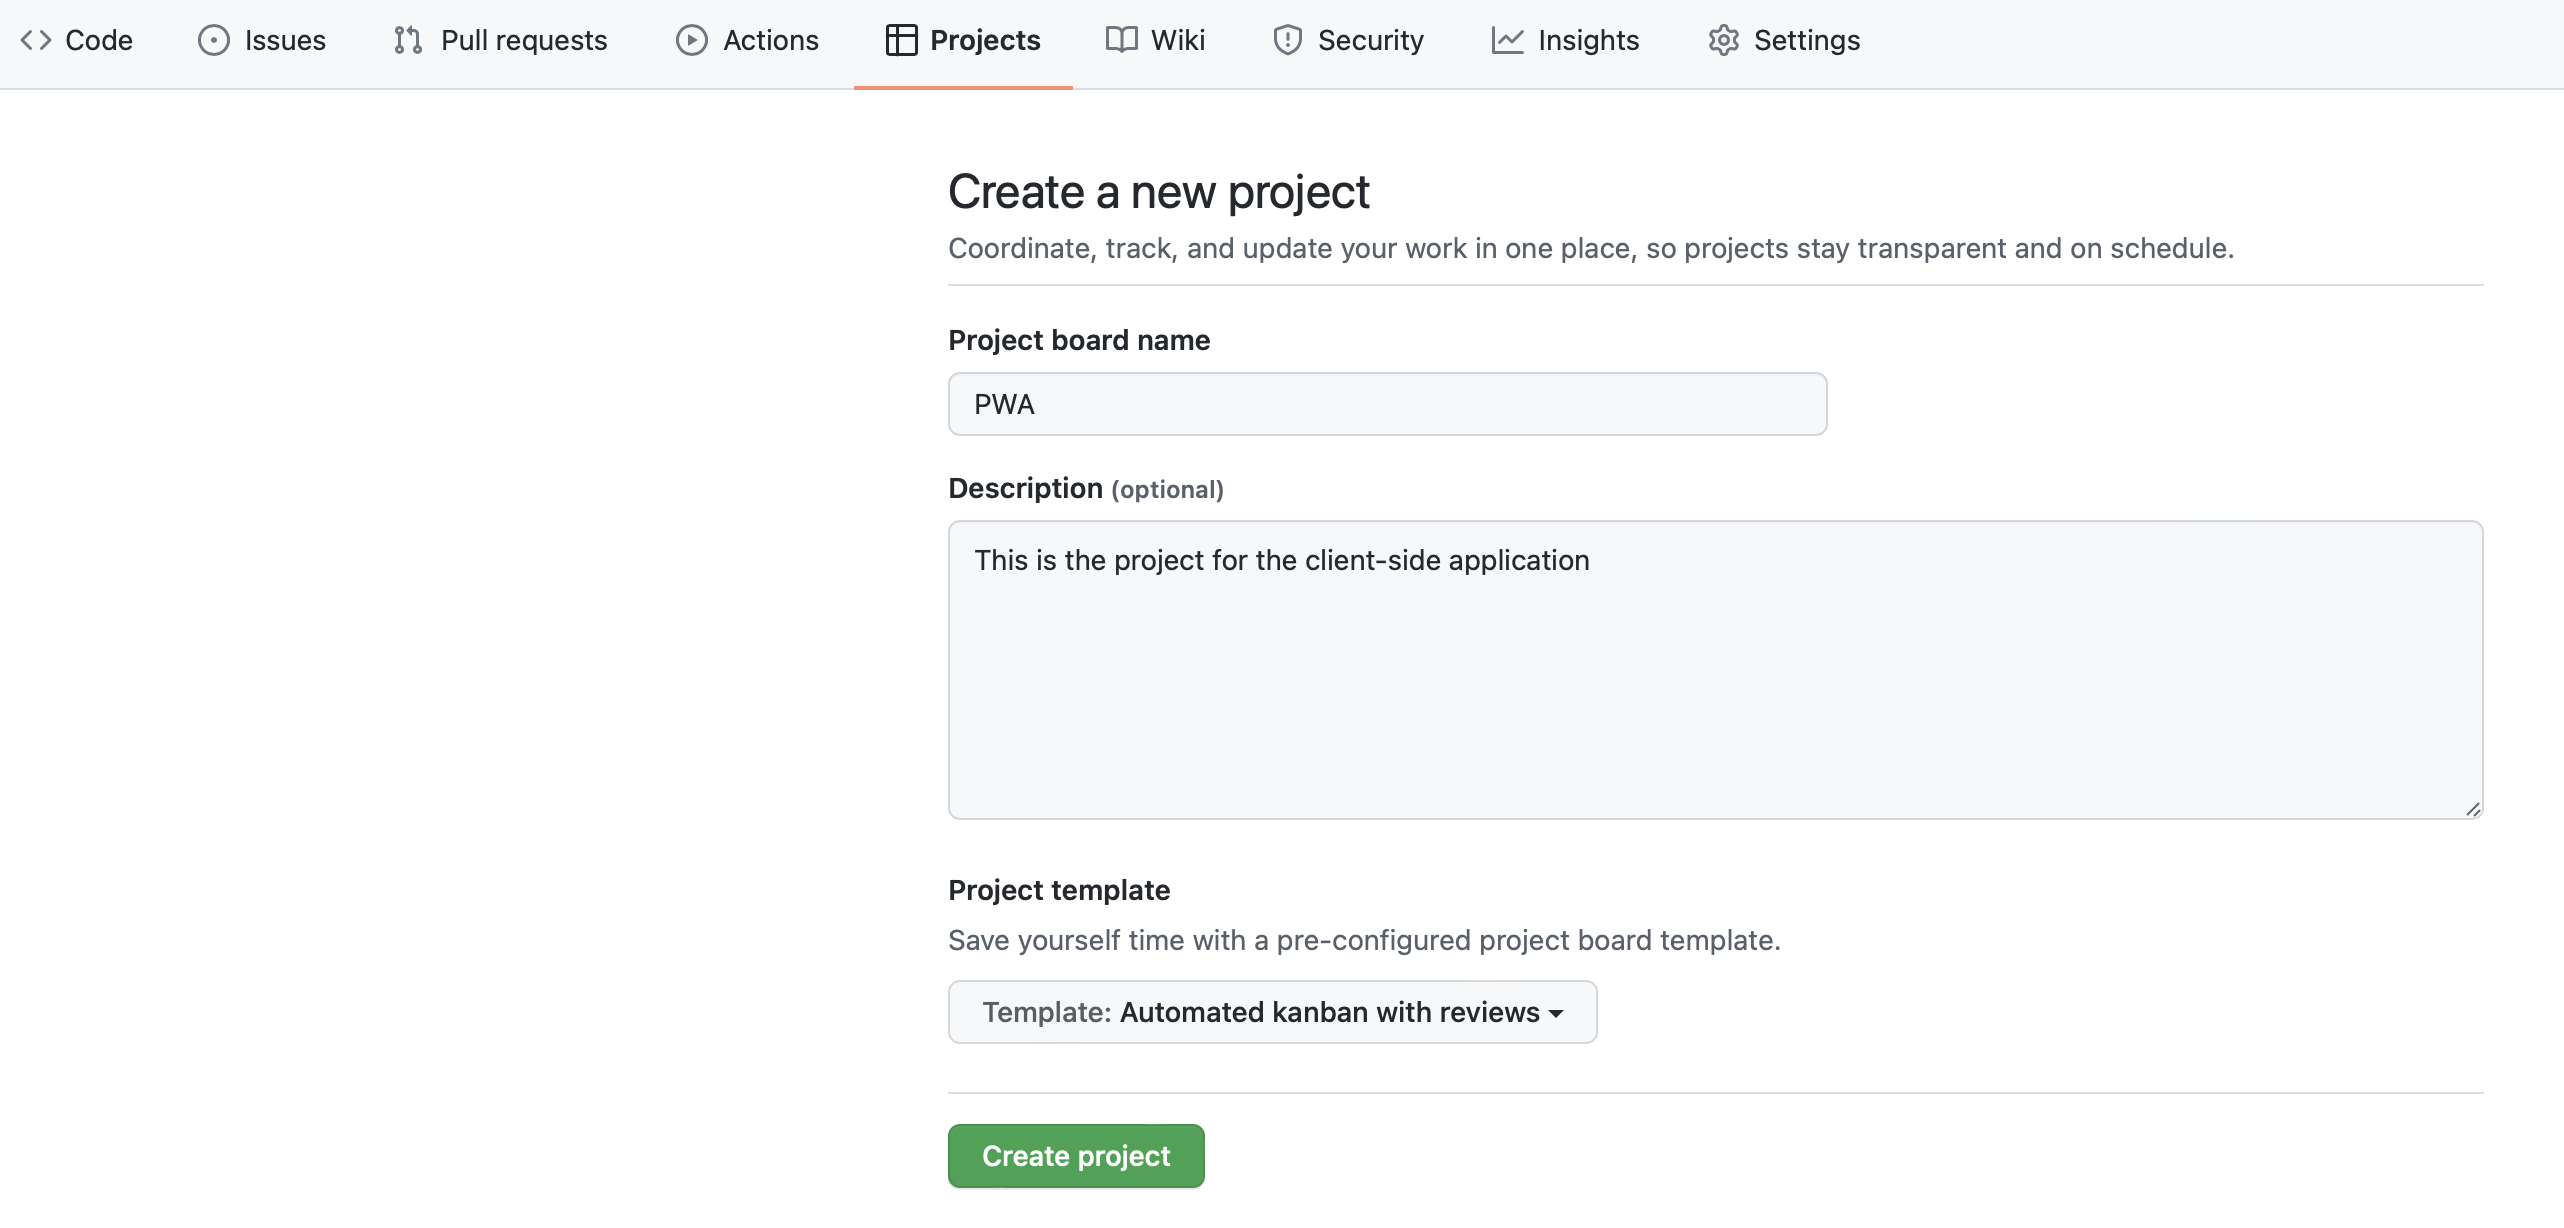
\includegraphics[width=\textwidth]{media/ProjectManagement/EnterProjectInfo.png}
    \caption{Eingabe der Projektinformationen}
    \label{fig:enterProjectInfo}
\end{figure}

\hthree{Erstellen eines Arbeitspaketes}

Im "Issues"-Tab lassen sich Meilensteine und Label erstellen. Durch Label kann man die Art der Arbeitspakete angeben. Diese können zum Beschreibung eine neue Funktionalität oder eine Fehlerbehebung sein. Um das Arbeitspaket selbst zu erstellen, muss ein Titel vergeben werden. Außerdem werden Meilenstein, Labels und ein oder mehrere Entwickler angegeben, welche dieses Arbeitspaket bearbeiten sollen. (Siehe Abbildung \ref{fig:createIssue})

\begin{figure}[H]
    \centering
    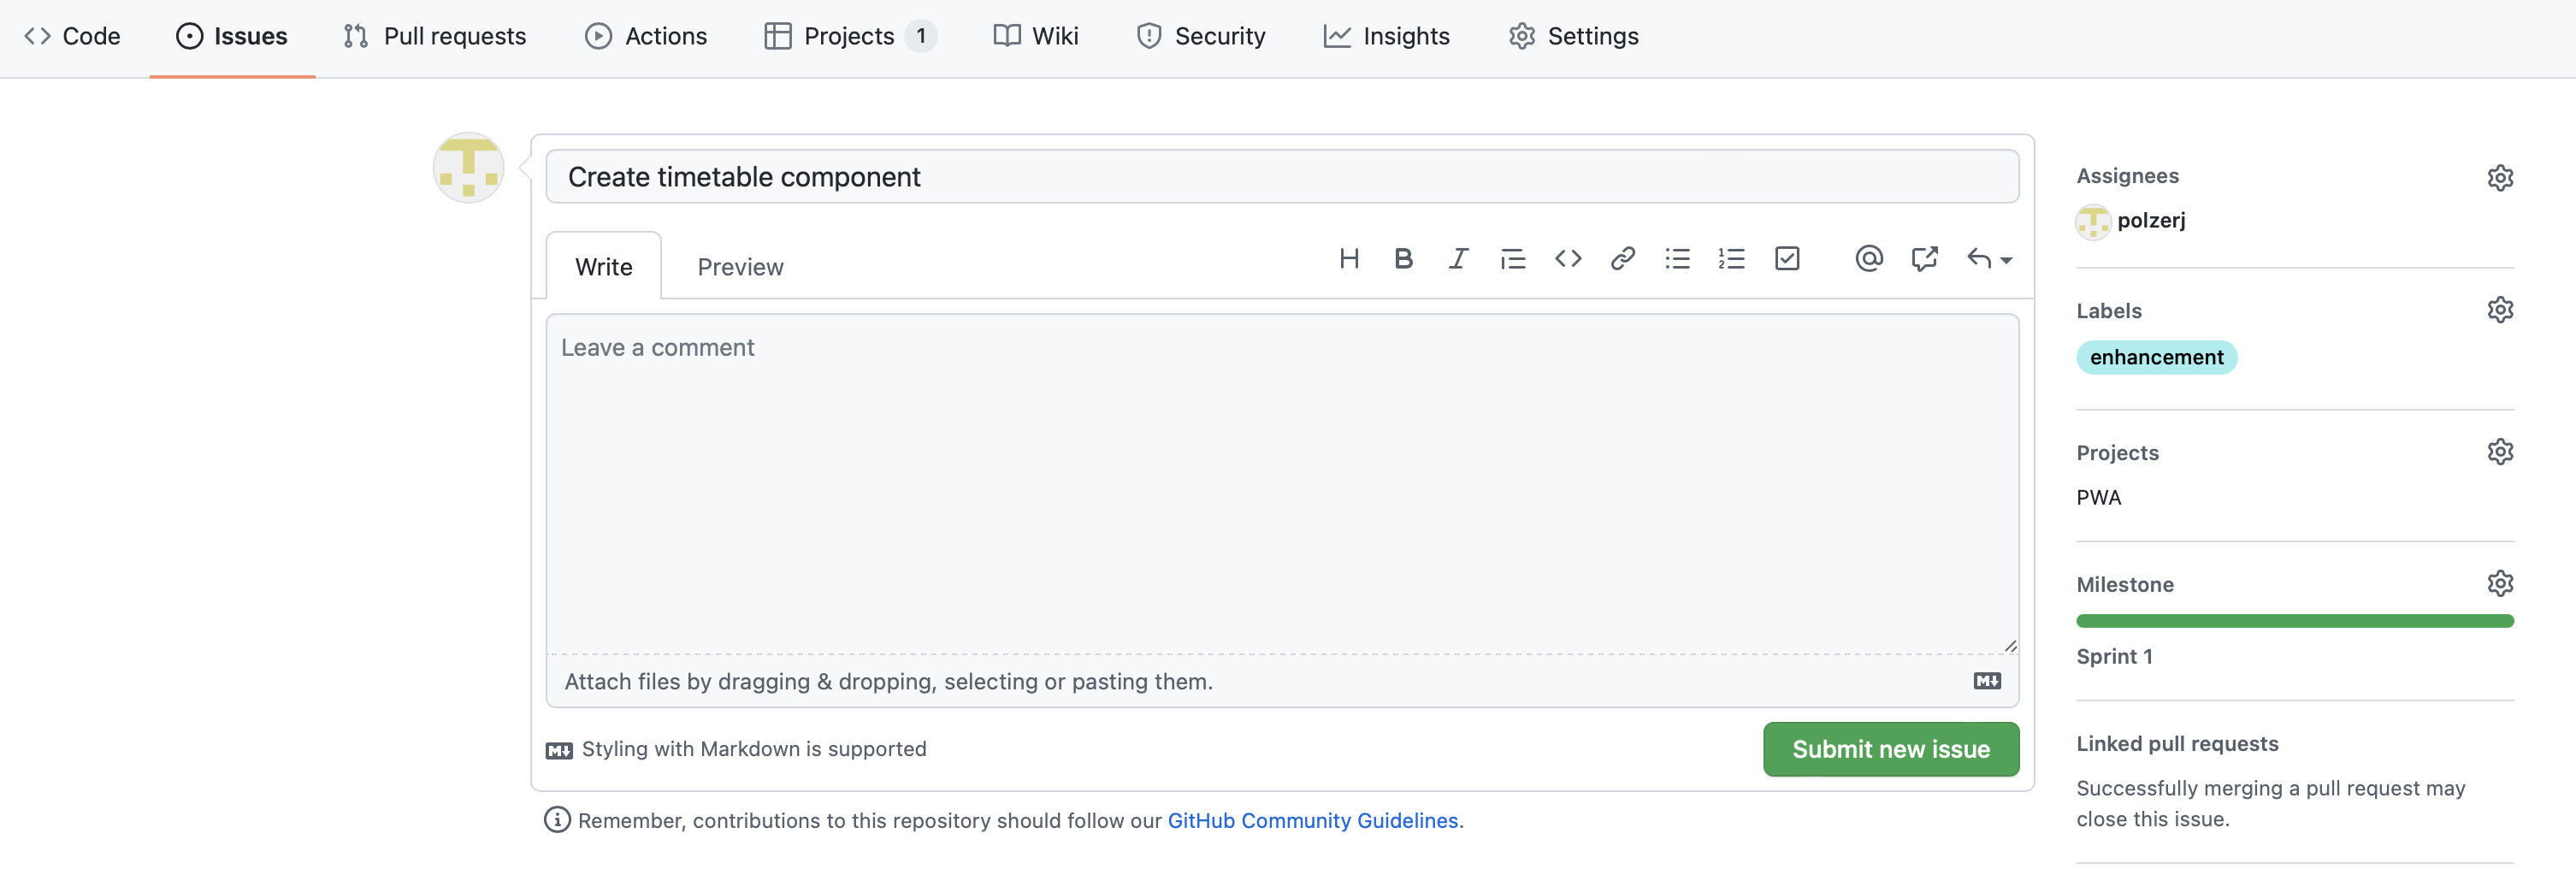
\includegraphics[width=\textwidth]{media/ProjectManagement/CreateIssue.png}
    \caption{Eingabe der Arbeitspaketinformationen}
    \label{fig:createIssue}
\end{figure}

\hthree{Arbeiten an einem Arbeitspaket}

%todo

\cite{GithubFS}